\chapter{Implementation}

\section{Lichess.org Puzzle Database}

\subsection{Overview}

This project requires access to various examples of chess puzzles with
pre-defined difficulties and themes. Fortunately, the \citet{lichessPuzzles}
puzzle database, which was mentioned in Section \ref{lichessPuzzlesSection},
provides approximately 3.8 million chess puzzles which have been generated from
user games played on Lichess. These puzzles are stored in FEN format, with a
reference to the game where they appeared. They also contain the solution as a
string moves, the tactics tags \citep{lichessXML}, and the puzzle rating, along
with other metadata.

An example puzzle string is shown below. This puzzle is also shown visually in
Figures \ref{puzzle1} and \ref{puzzle2}.

\begin{verbatim}
q3k1nr/1pp1nQpp/3p4/1P2p3/4P3/B1PP1b2/B5PP/5K2 b k - 0 17,
e8d7 a2e6 d7d8 f7f8,1760,80,83,72,mate mateIn2 middlegame short,
https://lichess.org/yyznGmXs/black#34,
Italian_Game Italian_Game_Classical_Variation
\end{verbatim}

\begin{figure}[H]
    \begin{minipage}{0.475\textwidth}
        \centering
        \chessboard[setfen=q3k1nr/1pp1nQpp/3p4/1P2p3/4P3/B1PP1b2/B5PP/5K2 b k - 0 17]
        \caption{\textbf{ZensAlviani -- desso2b}, lichess.org Blitz game, move 17.}
        \label{puzzle1}
    \end{minipage}
    \hspace{0.05\textwidth}
    \begin{minipage}{0.475\textwidth}
        \centering
        \chessboard[setfen=q5nr/1ppknQpp/3p4/1P2p3/4P3/B1PP1b2/B5PP/5K2 w - - 1 18]
        \caption{\textbf{ZensAlviani -- desso2b}, lichess.org Blitz game, move 18.
        Checkmate is imminent with \texttt{18.Be6+ Kd8 19.Qf8\#}.}
        \label{puzzle2}
    \end{minipage}
\end{figure}

Processing these is a trivial task with one small detail: the given FEN strings
are the state of the game right before the critical blunder is played by the
opposing site. This means the puzzle, as shown to the user, is the position
after the first move has been played. Fortunately, processing this data is made
simple with the python-chess library \citep{pythonChess}.

\subsection{Data Exploration}

The lichess puzzle database has approximately 3.8 million rated and tagged
chess puzzles. Initially, they were automatically processed
\citep{lichessTagger}, but were then refined with user feedback
\citep{lichessPuzzles}. This also allowed the puzzles to obtain a rating, which
is indicative of its difficulty \citep{lichessPuzzles}.

Overall, there are 60 various puzzle themes \citep{lichessXML}. Figure
\ref{dataThemeCounts} shows the counts of each theme in all of the contained
puzzles. It should be noted that some themes are mutually exclusive (a
checkmate puzzle cannot be both \emph{mate-in-one} and \emph{mate-in-two}).

The most common puzzle themes are the most general ones -- specifically
`short', `middlegame', and `endgame'. There is a lot of variation in how
frequent the various patterns are, which is a natural consequence of the game.

\begin{figure}
    \centering
    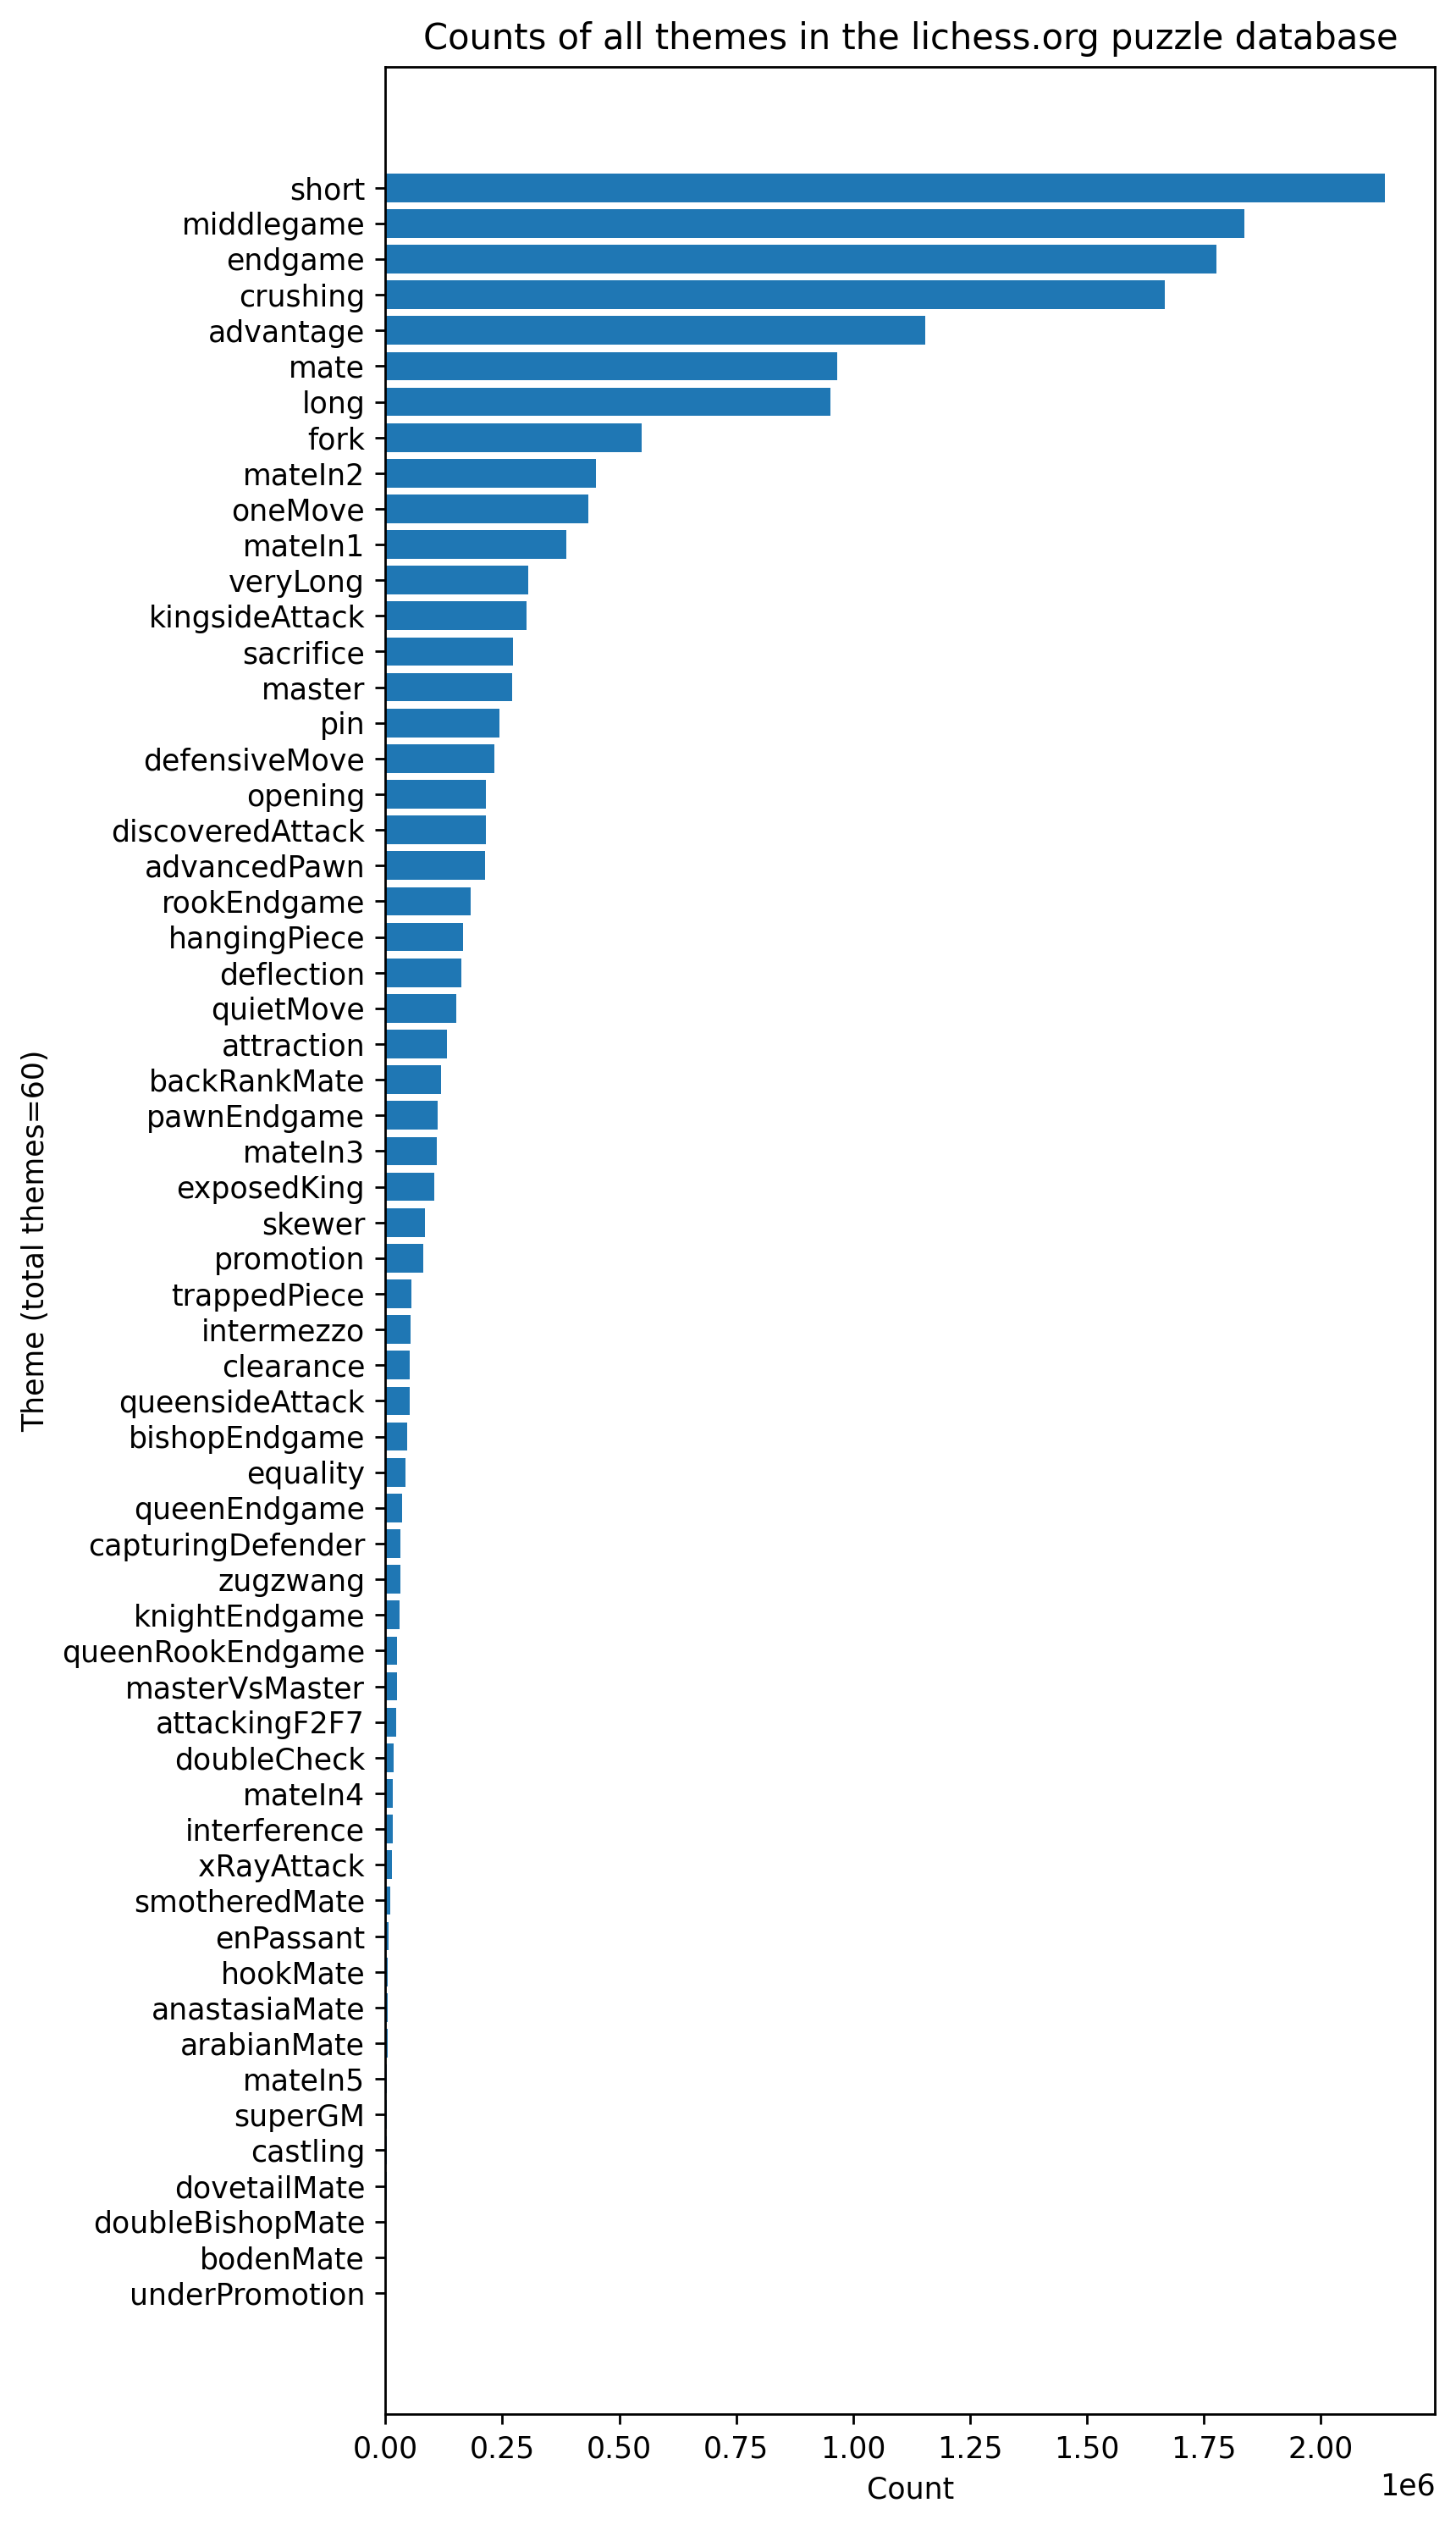
\includegraphics[width=0.9\linewidth]{project/img/puzzle_theme_counts.png}
    \caption{Frequency of puzzle themes in the lichess.org puzzle database.\cite{lichessPuzzles}}
    \label{dataThemeCounts}
\end{figure}

Figure \ref{dataHistogram} shows the distribution of ratings across the chess
puzzles. It should be noted that these ratings are only appropriate within this
dataset, and cannot be compared to ratings of puzzles on other chess websites.
The puzzle ratings are quite symmetric about the mean, and this is of course a
result of the Glicko2 rating system, developed by \citet{glicko}.

When analysing the rating distribution by theme, an expected behaviour occurs.
Some chess tactics patterns are considerably simpler to spot, meaning a weaker
player is able to solve the puzzle with that theme. Therefore some puzzle
themes, \emph{back-rank mate}, for example, have lower-rated puzzles when
compared to puzzles featuring a \emph{trapped piece} or \emph{defensive
move}.\footnote{Notoriously difficult for humans, who are usually much better
at aggression than defense.\footnotemark}\footnotetext{In chess.}

Figures \ref{puzzle3} and \ref{puzzle4} show examples of some puzzles with
these themes.

\begin{figure}[H]
    \begin{minipage}{0.475\textwidth}
        \centering
        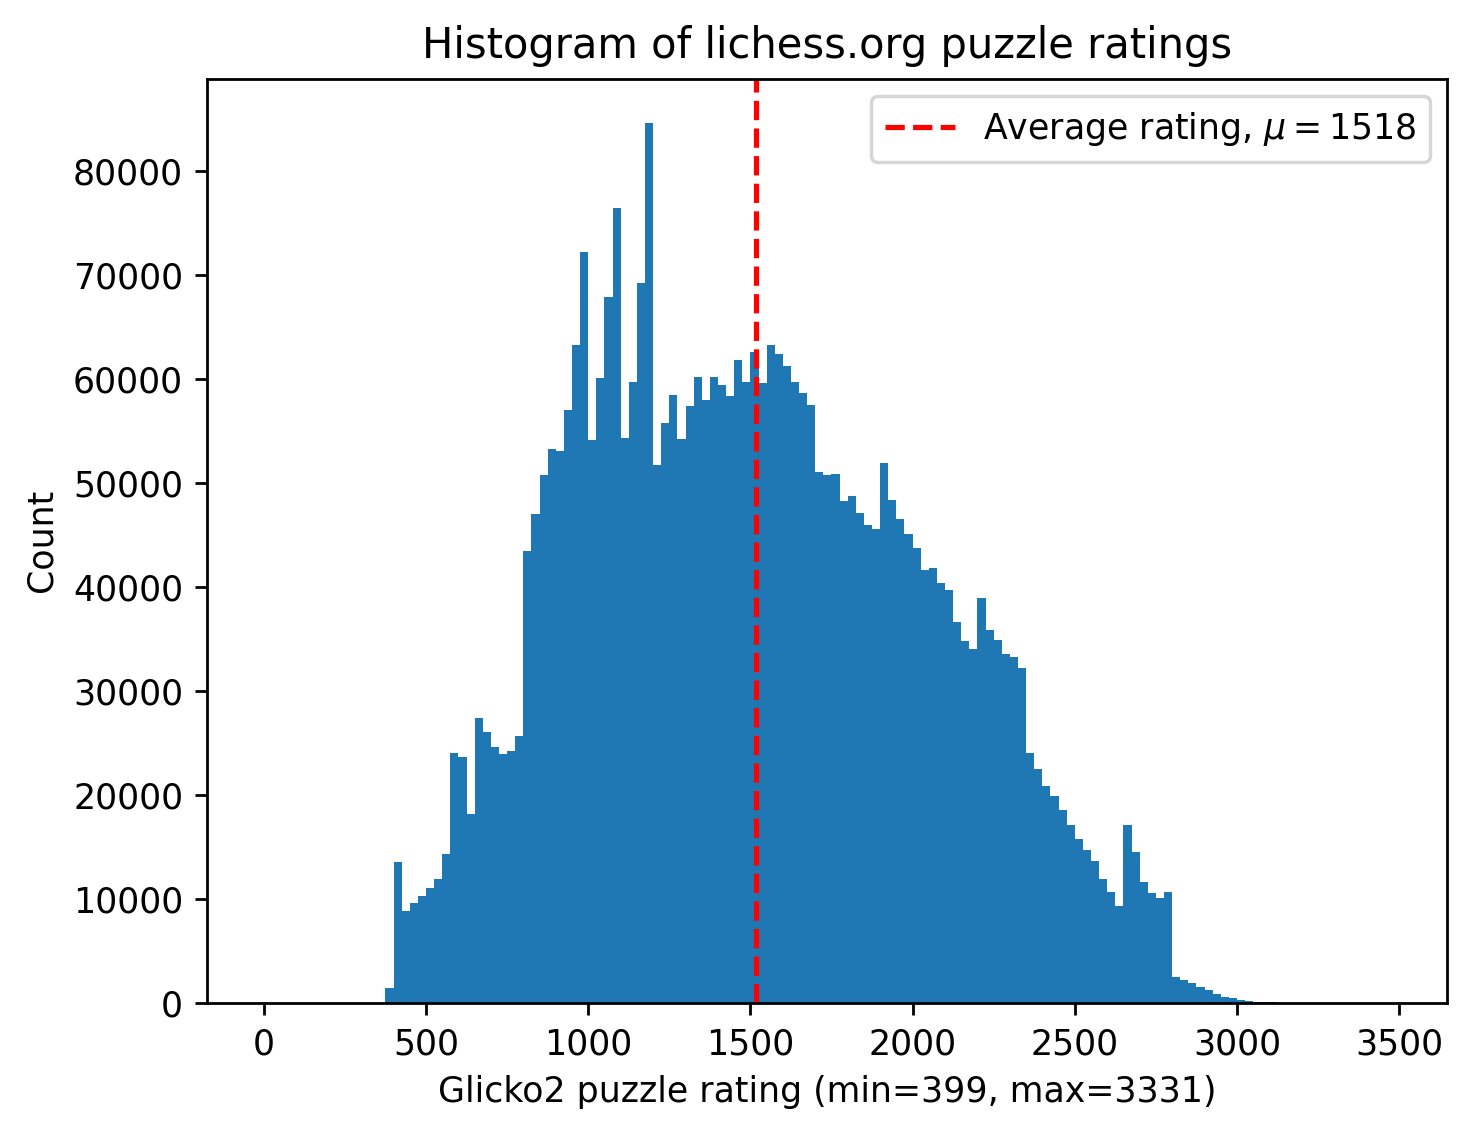
\includegraphics[width=\textwidth]{project/img/puzzle_histogram.png}
        \caption{Distribution of Lichess puzzle ratings.}
        \label{dataHistogram}
    \end{minipage}
    \hspace{0.05\textwidth}
    \begin{minipage}{0.475\textwidth}
        \centering
        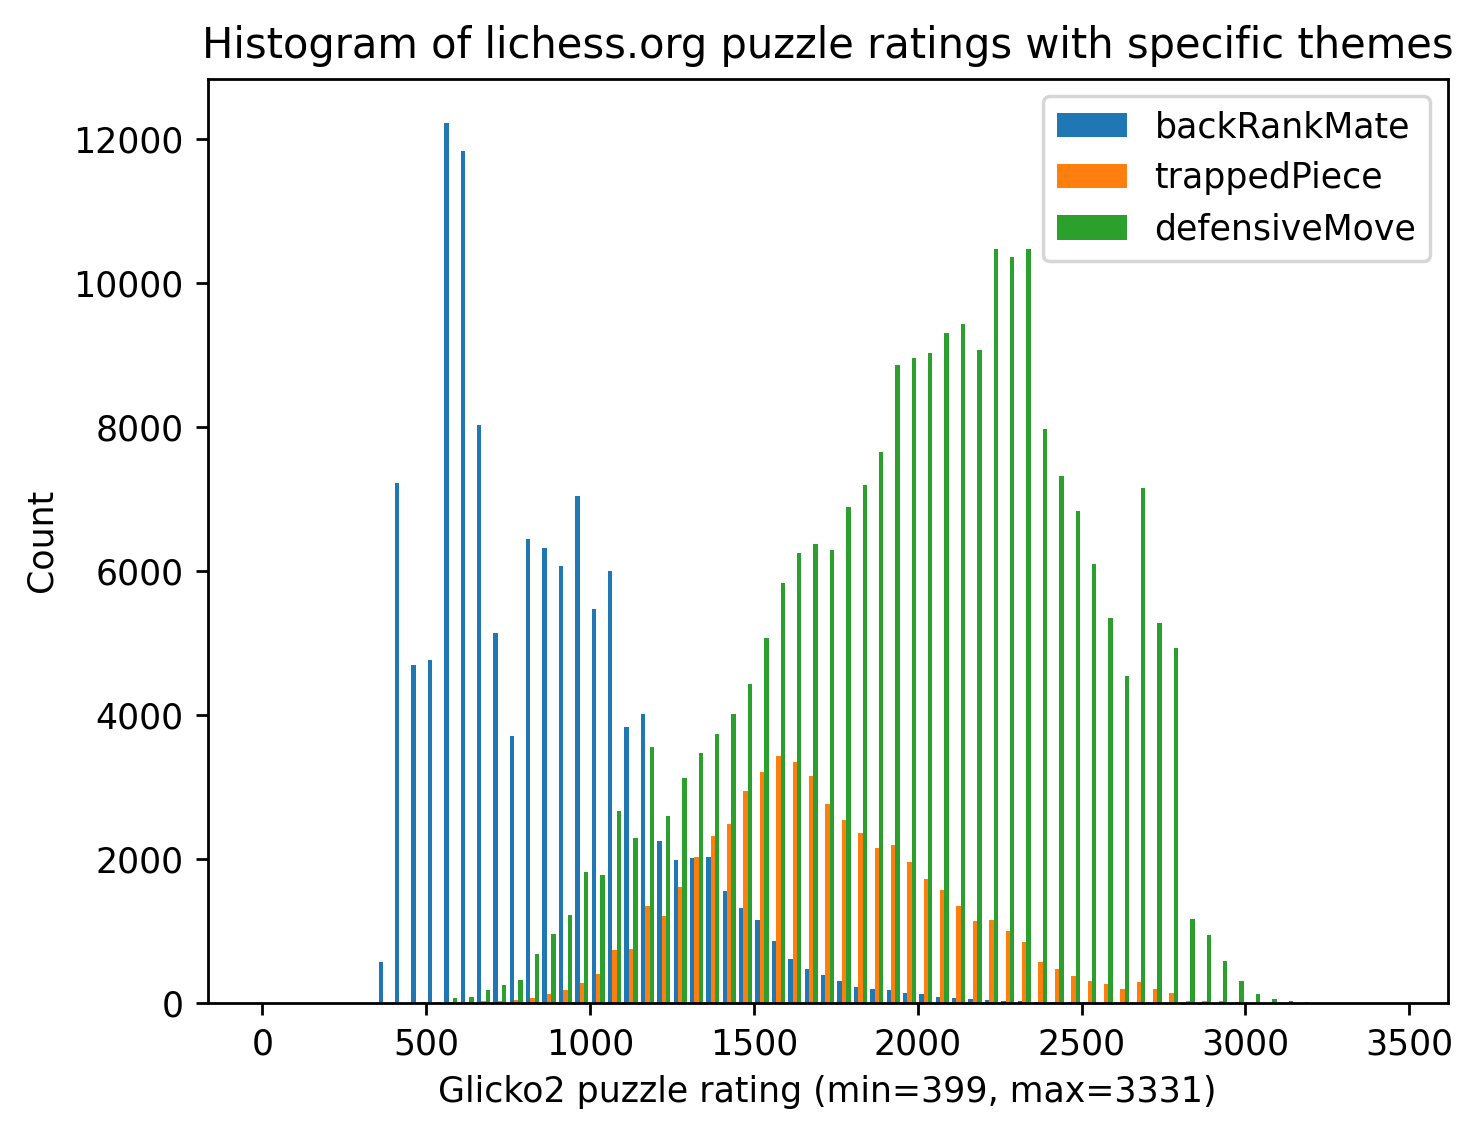
\includegraphics[width=\textwidth]{project/img/puzzle_theme_histograms.png}
        \caption{Distribution of Lichess puzzle ratings with a specific theme.}
        \label{dataThemeHistogram}
    \end{minipage}
\end{figure}

\begin{figure}[H]
    \begin{minipage}{0.475\textwidth}
        \centering
        \chessboard[setfen=6k1/5ppp/r1p5/p1n1rP2/8/2P2N1P/2P3P1/3R2K1 w - - 0 22]
        \caption{\textbf{Kenan2345 -- gandie}, lichess.org Blitz game, move 22. 
        Black loses to \texttt{22.Rd8+}.}
        \label{puzzle3}
    \end{minipage}
    \hspace{0.05\textwidth}
    \begin{minipage}{0.475\textwidth}
        \centering
        \chessboard[setfen=2rq1rk1/7p/1n4pb/1R2Q3/pPpP1P2/P1B5/3N2PP/2R3K1 b - - 0 31]
        \caption{\textbf{mhabib -- Sarg0n}, lichess.org Blitz game, move 31. White loses his queen after \texttt{31...Re38}, as the queen has no safe squares to escape to.}

        \label{puzzle4}
    \end{minipage}
\end{figure}

\section{The Machine Learning Approach}

\subsection{Introduction}

In this section, we describe, analyse, and evaluate a novel approach to the
specific problem of chess puzzle classification, inspired by the recent
unstoppable advancements in the field of natural language processing.

Earlier, we highlighted a number of papers which seek to find new ways to build
on the naive bitboard representation \citep{middleGamePatterns, chessCNN,
chess2vec} by exploring new embeddings for chess pieces and chess board
squares. All three of the publications make the crucial point that chess pieces
influence each other on the board, and this has to be taken into account,
whether it is by creating extra features to represent pins and central square
control \citep{chessCNN}, open files and attack squares
\citep{middleGamePatterns}, or the hash of the entire chess board
\cite{chess2vec}.

Continuing along the `chess board as a $N\times64$ vector' path and, given how
puzzle tactics rely on the interaction of pieces' locations and attack squares,
it seems natural to explore whether the transformer architecture, as described
in the infamous paper `Attention is All you Need' \citep{attention}, can help
extract patterns from static chess positions, which can then be used in the
downstream task of puzzle classification and difficulty rating. Figure
\ref{attentionLinks}, taken from this paper, shows how words/tokens can
influence each other in the transformer encoder. At a high level, chess pieces
and squares interact in a similar way on the chess board -- see Figure
\ref{chessPuzzleLinks} for an example.

Applying transformers to chess has been done before by
\citet{chessTransformer}, but as far as we are aware, treating individual chess
board squares as embeddings of tokens/words has not been previously explored.

\begin{figure}[H]
    \begin{minipage}{0.425\textwidth}
        \centering
        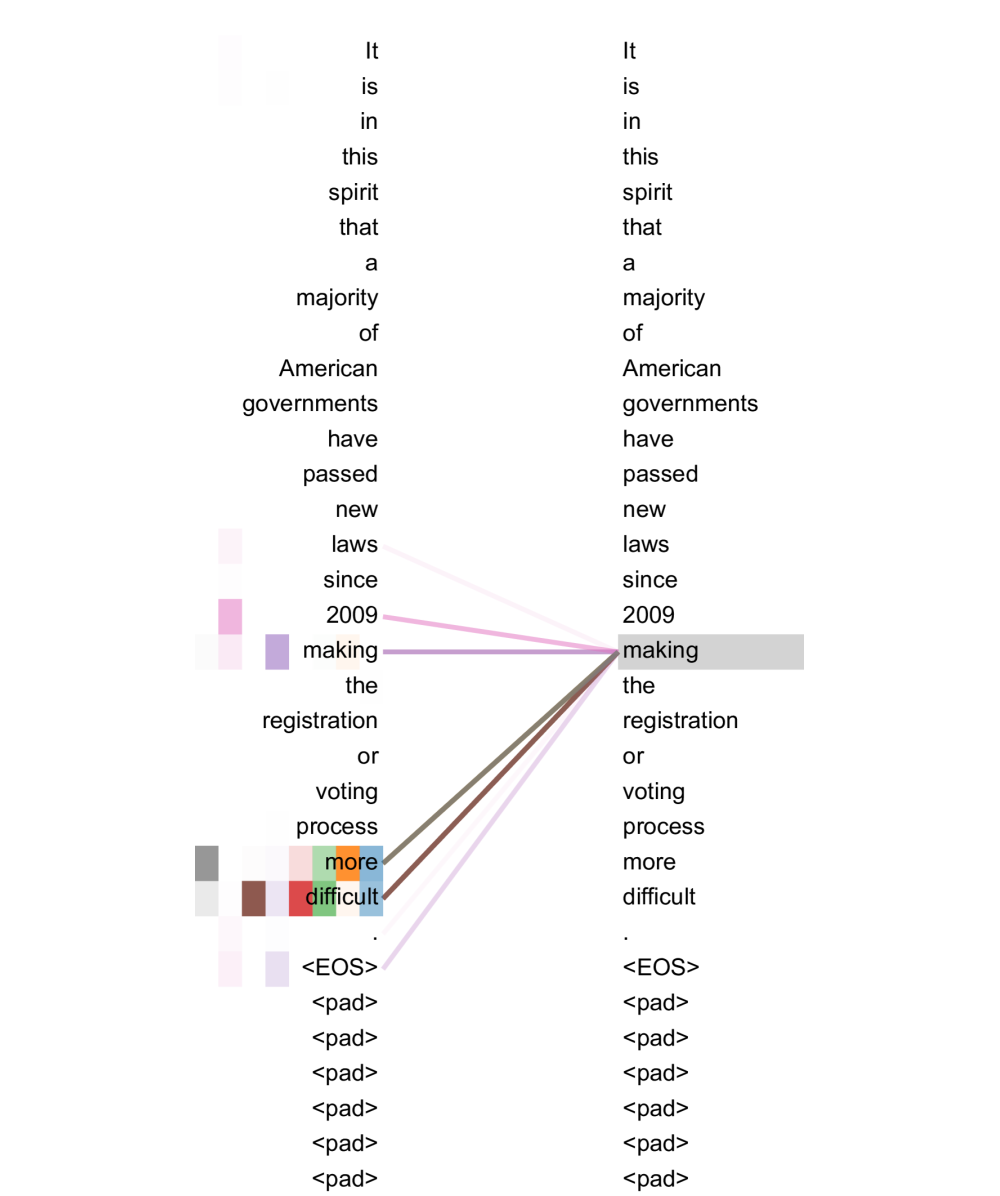
\includegraphics[width=\textwidth]{project/img/attention.png}
        \caption{Example of attention mechanism in the encoder. Taken from `Attention Is All You Need' \citep{attention}.}
        \label{attentionLinks}
    \end{minipage}
   \hspace{0.05\textwidth}
    \begin{minipage}{0.475\textwidth}
        \centering
        \chessboard[setfen=r3r1n1/bp6/p2p2kp/3N4/2P3n1/1PQ3Pq/P4P2/4RRK1 w - - 0 1,
                    pgfstyle=border,markfields={d5},
                    pgfstyle=straightmove,markmoves={f4-g6,f4-h3,c7-a8,c7-e8,d5-c7,d5-f4},
                    pgfstyle=color,opacity=0.5,color=blue,markfields={f4,c7},
                    pgfstyle=color,opacity=0.5,color=red,markfields={h3,g6,a8,e8}]
        \caption{Example of a relationship between chess pieces.}

        \label{chessPuzzleLinks}
    \end{minipage}
\end{figure}

\subsection{Data Preparation}

We formulate the problem of chess puzzle analysis as a multi-label
classification problem. Given a chess puzzle position in bitboard format,
i.e.\@ a $12\times8\times8$ binary tensor, we aim to predict a binary indicator
vector which encodes the labels of the puzzle themes. Slightly more formally,
the element $B[z, x, y]$ of bitboard $B$ is $1$ iff there is a piece $z \in
\{\texttt{p}, \texttt{P}, \texttt{n}, \texttt{N}, \texttt{b}, \texttt{B},
\texttt{r}, \texttt{R}, \texttt{q}, \texttt{Q}, \texttt{k},
\texttt{K}\}$\footnote{FEN-inspired -- white pieces are uppercas\texttt{e},
black pieces are lowercase.} at rank $x \in \{\texttt{1}, \texttt{2},
\texttt{3}, \texttt{4}, \texttt{5}, \texttt{6}, \texttt{7}, \texttt{8}\}$},
file $y \in \{\texttt{a}, \texttt{b}, \texttt{c}, \texttt{d}, \texttt{e},
\texttt{f}, \texttt{g}, \texttt{h}\}$.

Given a dataset with $N$ distinct puzzle labels ($N=60$ for the Lichess puzzle
database), we assign each label an index $i$ and form a binary $N$-dimensional
vector $x$ such that $x[i]=1$ iff the puzzle is labelled with that label. This
is a common technique to reduce a multi-label classification into a more
tractable problem.

To make learning easier (and to decrease implementation complexity), we
transform all chess positions to be from the perspective of White. This has
negligible additional overhead, as it requires a simple mirror and has great
benefits, as the model no longer needs to distinguish between white-to-move and
black-to-move puzzles.

\subsection{Model Architecture}

\begin{figure}[H]
        \centering
        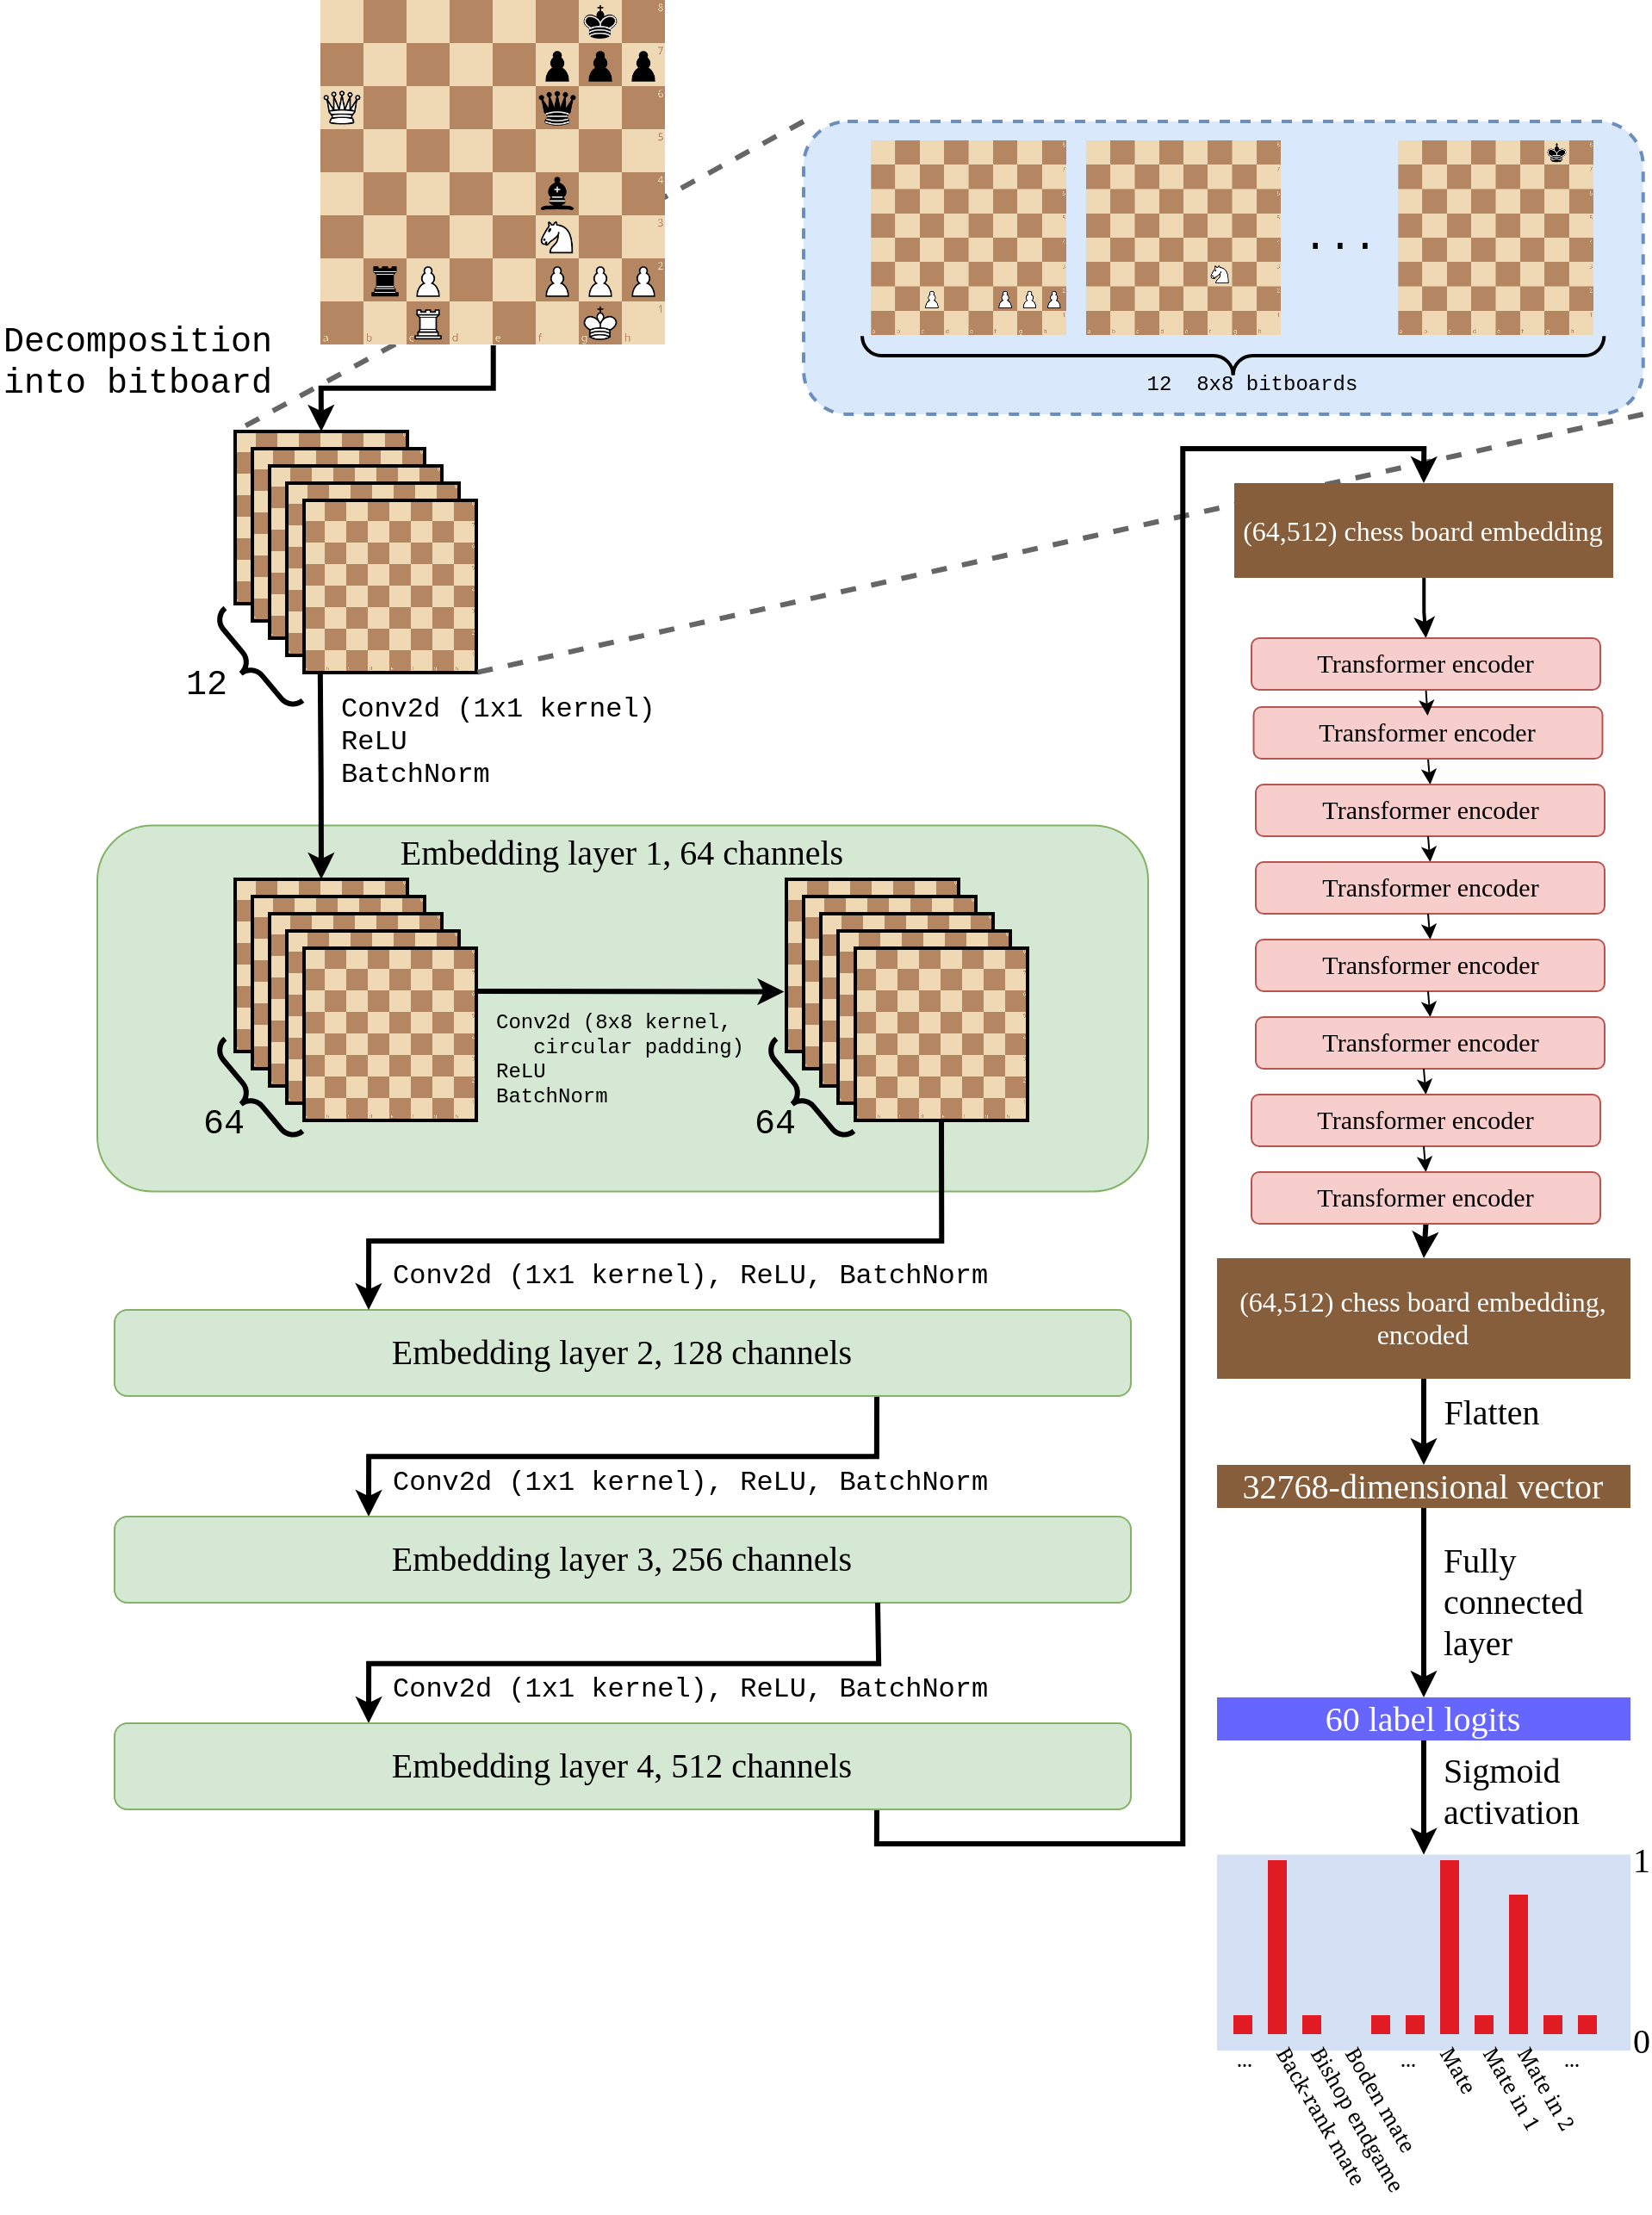
\includegraphics[width=\textwidth]{project/img/ml_diagram.png}
        \caption{High-level overview of the model architecture. Transformer encoder diagram taken from `Attention Is All You Need' \citep{attention}.}
        \label{MLDiagram}
\end{figure}


\section{The Graph-Based Approach}

\subsection{Introduction}

In this section, we propose a different novel approach to puzzle
classification, focusing on unsupervised puzzle clustering and defining a
distance function between various chess puzzles.

This method seeks to combine and build upon two approaches seen in the above
literature review: the tree-based puzzle difficulty classification
\citep{chessTrees} covered in Section \ref{chessTreesOverview} and chess
position similarity using dynamic features \citep{chessMotifs} covered in
Section \ref{chessMotifsOverview}. We hypothesise that by combining these
approaches to construct meaningful search trees with additional node labels,
defining a distance function for individual chess moves, and applying a
labelled tree edit distance function \citep{editDistTrees}, we would be able to
calculate `closeness' of chess puzzles. This could also help refine the work of
\citet{chessTrees} by finer segregating puzzles by difficulty level.

\subsection{High-level overview}

As explored by \citet{chessTrees}, `meaningful search trees' have predictive
possibility of a puzzle's difficulty. These trees are constructed by analysing
powerful moves that either gain, or at least do not worsen a side's position. 

By additionally labelling these trees with move information, we hope to build
upon this work. To demonstrate the intuition behind this idea, there are two
labelled search trees shown in Figures \ref{tree1}, \ref{tree2}. These are the
search trees for positions in Figures \ref{chess5}, \ref{chess6} which feature
a identical and complex tactical motif. 

In the following trees, algebratic notation of the moves is shown, along with 4
slash-delimited integers, which correspond to: pieces attacked, pieces
defended, number of attackers, number of defenders.\footnote{As the moves must
be legal, this means a king move will never have any attackers, and any
check/mate will have at least 1 piece attacked -- the enemy king.} Whilst the 2
trees do not look similar visually (their size being the main problem), the
first 3 plies are very similar. 

\begin{figure}[H]
    \begin{minipage}{0.475\textwidth}
        \centering
        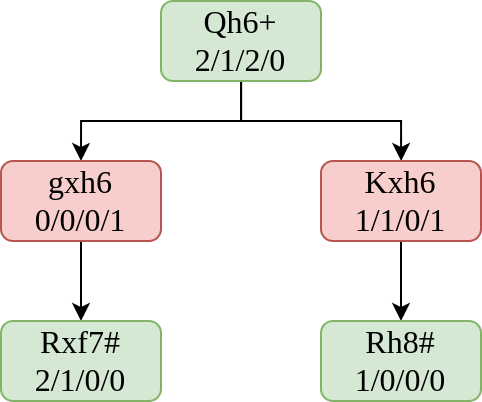
\includegraphics[width=\textwidth]{project/img/trees/1.drawio.png}
        \caption{Labelled search tree for game in \ref{chess5}}
        \label{tree1}
    \end{minipage}
    \hspace{0.05\textwidth}
    \begin{minipage}{0.475\textwidth}
        \centering
        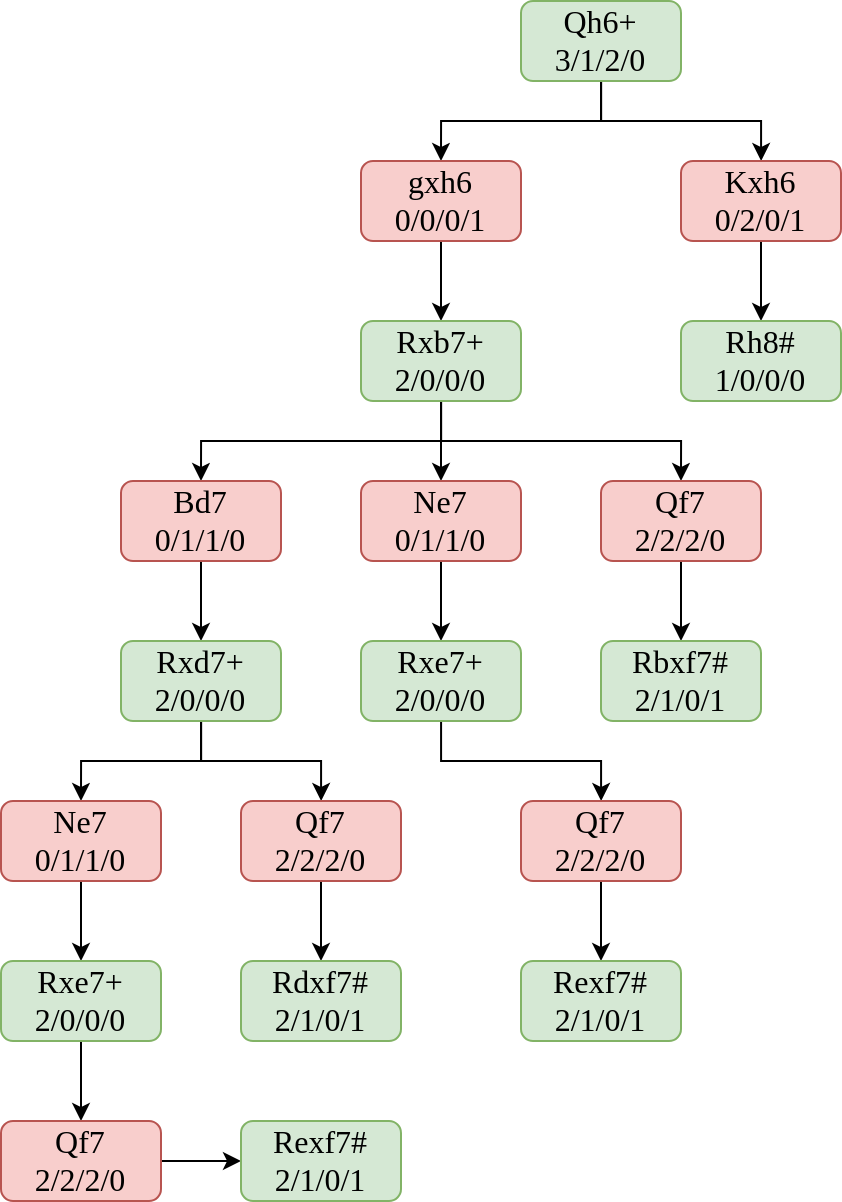
\includegraphics[width=\textwidth]{project/img/trees/2.drawio.png}
        \caption{Labelled search tree for game in \ref{chess6}}
        \label{tree2}
    \end{minipage}
\end{figure}

In Figures \ref{puzzle5}, \ref{puzzle6} are two chess puzzles from the paper
`Automatic Recognition of Similar Chess Motifs' \citep{chessMotifs}. Despite
their visual difference, these both feature a rook sacrifice, and an imminent
queen checkmate helped by the powerful light-squared bishop. This similarity is
not immediately obvious, but the search trees for these puzzles is almost
identical, except for minor attacker/defender discrepancies. The trees are
shown in Figures \ref{tree3}, \ref{tree4}. These puzzles were already
successfully grouped by \citet{chessMotifs}.

\begin{figure}[H]
    \begin{minipage}{0.475\textwidth}
        \centering
        \chessboard[setfen= 4r1k1/1b3pp1/4p3/p2r4/7R/2B1Q1PP/P1P1RP1K/1q6 w - -
        0 1]
        \caption{Taken from `Automatic Recognition of Similar Chess Motifs'
        \citep{chessMotifs}. White mates in 3 (\texttt{1.Rh8+ Kxh8 2.Qh6+ Kg8
        3.Qxg7#}).}
        \label{puzzle5}
    \end{minipage}
    \hspace{0.05\textwidth}
    \begin{minipage}{0.475\textwidth}
        \centering
        \chessboard[setfen=r5k1/5pp1/8/3p3R/2q4P/PbB2P2/1P1Q2P1/K7 w q - 0 1]
            \caption{Also taken from `Automatic Recognition of Similar Chess
            Motifs' \citep{chessMotifs}. White mates in 3 with the same moves
            as the puzzle on the left.}
        \label{puzzle6}
    \end{minipage}
\end{figure}

\begin{figure}[H]
    \begin{minipage}{0.475\textwidth}
        \centering
        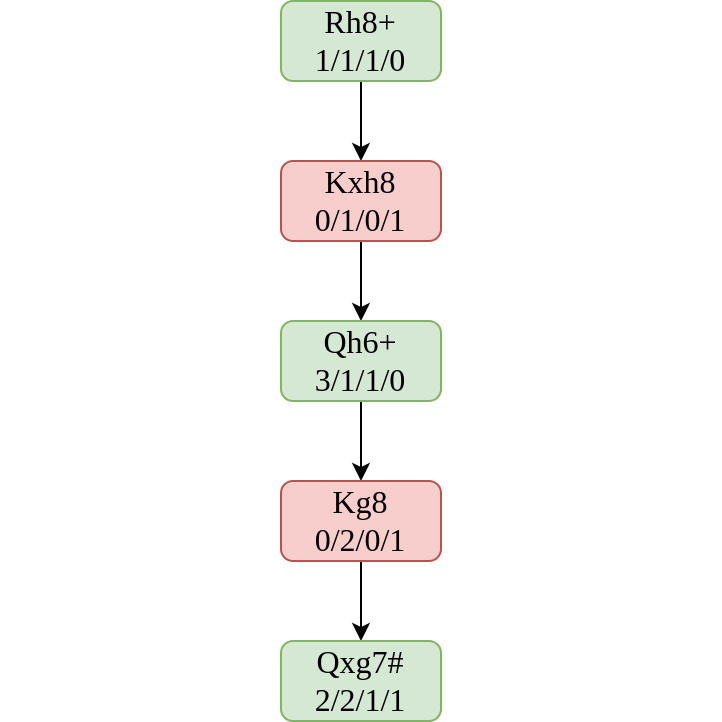
\includegraphics[width=\textwidth]{project/img/trees/3.drawio.png}
        \caption{Labelled search tree for game in Figure \ref{puzzle5}.}
        \label{tree3}
    \end{minipage}
    \hspace{0.05\textwidth}
    \begin{minipage}{0.475\textwidth}
        \centering
        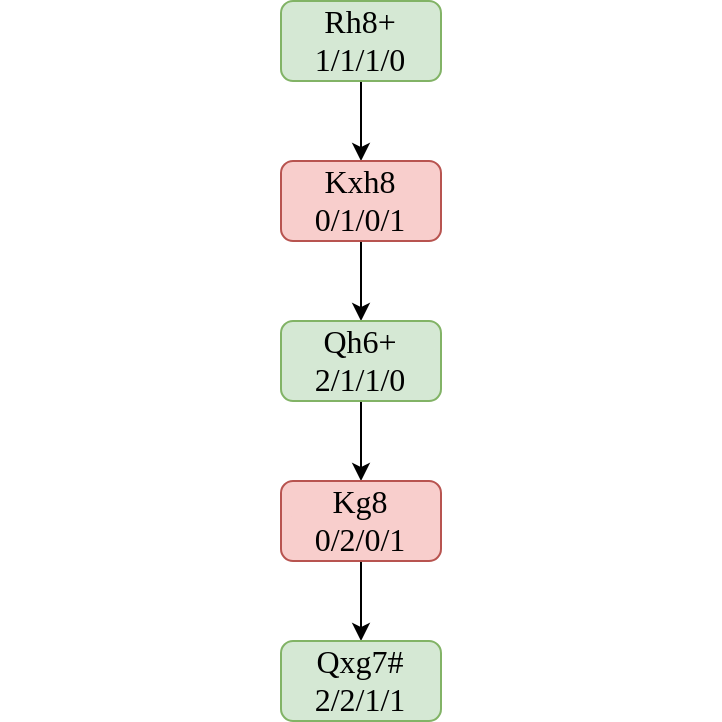
\includegraphics[width=\textwidth]{project/img/trees/4.drawio.png}
        \caption{Labelled search tree for game in Figure \ref{puzzle6}.}
        \label{tree4}
    \end{minipage}
\end{figure}

